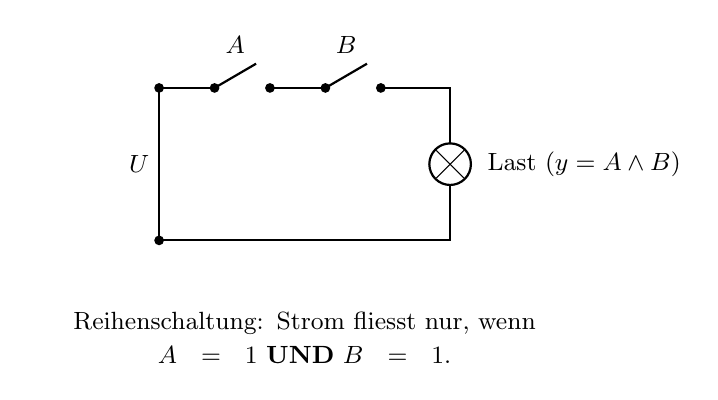
\begin{tikzpicture}[scale=0.88, >=stealth]
    \draw[thick] (0,0) -- (0,2.2) -- (0.8,2.2);
    \node[left, font=\small] at (0,1.1) {$U$};
    \fill (0,0) circle (2pt); \fill (0,2.2) circle (2pt);

    % Schalter A
    \fill (0.8, 2.2) circle (2pt);
    \draw[thick] (0.8, 2.2) -- (1.4, 2.55);
    \node[above, font=\small] at (1.1, 2.55) {$A$};
    \fill (1.6, 2.2) circle (2pt);
    \draw[thick] (1.6, 2.2) -- (2.4, 2.2);

    % Schalter B
    \fill (2.4, 2.2) circle (2pt);
    \draw[thick] (2.4, 2.2) -- (3.0, 2.55);
    \node[above, font=\small] at (2.7, 2.55) {$B$};
    \fill (3.2, 2.2) circle (2pt);
    \draw[thick] (3.2, 2.2) -- (4.2, 2.2) -- (4.2, 1.4);

    % Lampe y
    \draw[thick] (4.2, 1.1) circle (0.3);
    \draw (4.0, 0.9) -- (4.4, 1.3);
    \draw (4.0, 1.3) -- (4.4, 0.9);
    \node[right, font=\small] at (4.6, 1.1) {Last ($y = A \land B$)};
    \draw[thick] (4.2, 0.8) -- (4.2, 0) -- (0,0);

    \node[align=center, font=\small, text width=6.8cm, anchor=north] at (2.1, -0.9) {Reihenschaltung: Strom fliesst nur, wenn\\[1pt]\textbf{$A=1$ UND $B=1$}.};
\end{tikzpicture}
